% Options for packages loaded elsewhere
\PassOptionsToPackage{unicode}{hyperref}
\PassOptionsToPackage{hyphens}{url}
%
\documentclass[
]{article}
\usepackage{lmodern}
\usepackage{amssymb,amsmath}
\usepackage{ifxetex,ifluatex}
\ifnum 0\ifxetex 1\fi\ifluatex 1\fi=0 % if pdftex
  \usepackage[T1]{fontenc}
  \usepackage[utf8]{inputenc}
  \usepackage{textcomp} % provide euro and other symbols
\else % if luatex or xetex
  \usepackage{unicode-math}
  \defaultfontfeatures{Scale=MatchLowercase}
  \defaultfontfeatures[\rmfamily]{Ligatures=TeX,Scale=1}
\fi
% Use upquote if available, for straight quotes in verbatim environments
\IfFileExists{upquote.sty}{\usepackage{upquote}}{}
\IfFileExists{microtype.sty}{% use microtype if available
  \usepackage[]{microtype}
  \UseMicrotypeSet[protrusion]{basicmath} % disable protrusion for tt fonts
}{}
\makeatletter
\@ifundefined{KOMAClassName}{% if non-KOMA class
  \IfFileExists{parskip.sty}{%
    \usepackage{parskip}
  }{% else
    \setlength{\parindent}{0pt}
    \setlength{\parskip}{6pt plus 2pt minus 1pt}}
}{% if KOMA class
  \KOMAoptions{parskip=half}}
\makeatother
\usepackage{xcolor}
\IfFileExists{xurl.sty}{\usepackage{xurl}}{} % add URL line breaks if available
\IfFileExists{bookmark.sty}{\usepackage{bookmark}}{\usepackage{hyperref}}
\hypersetup{
  pdftitle={linear norm plot},
  pdfauthor={Joshua},
  hidelinks,
  pdfcreator={LaTeX via pandoc}}
\urlstyle{same} % disable monospaced font for URLs
\usepackage[margin=1in]{geometry}
\usepackage{graphicx,grffile}
\makeatletter
\def\maxwidth{\ifdim\Gin@nat@width>\linewidth\linewidth\else\Gin@nat@width\fi}
\def\maxheight{\ifdim\Gin@nat@height>\textheight\textheight\else\Gin@nat@height\fi}
\makeatother
% Scale images if necessary, so that they will not overflow the page
% margins by default, and it is still possible to overwrite the defaults
% using explicit options in \includegraphics[width, height, ...]{}
\setkeys{Gin}{width=\maxwidth,height=\maxheight,keepaspectratio}
% Set default figure placement to htbp
\makeatletter
\def\fps@figure{htbp}
\makeatother
\setlength{\emergencystretch}{3em} % prevent overfull lines
\providecommand{\tightlist}{%
  \setlength{\itemsep}{0pt}\setlength{\parskip}{0pt}}
\setcounter{secnumdepth}{-\maxdimen} % remove section numbering
\usepackage{booktabs}
\usepackage{longtable}
\usepackage{array}
\usepackage{multirow}
\usepackage{wrapfig}
\usepackage{float}
\usepackage{colortbl}
\usepackage{pdflscape}
\usepackage{tabu}
\usepackage{threeparttable}
\usepackage{threeparttablex}
\usepackage[normalem]{ulem}
\usepackage{makecell}
\usepackage{xcolor}

\title{linear norm plot}
\author{Joshua}
\date{15/05/2020}

\begin{document}
\maketitle

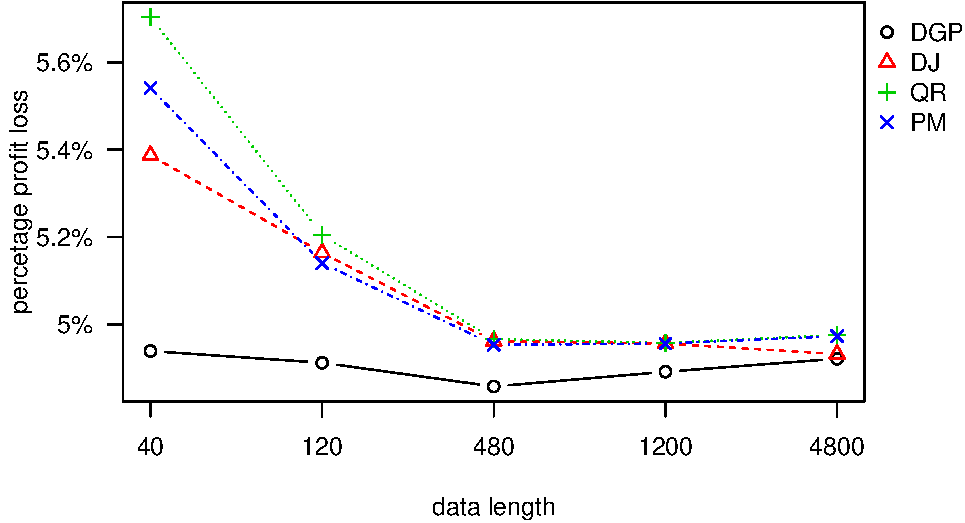
\includegraphics{linear-norm-plot_files/figure-latex/ppl0.5-1.pdf}

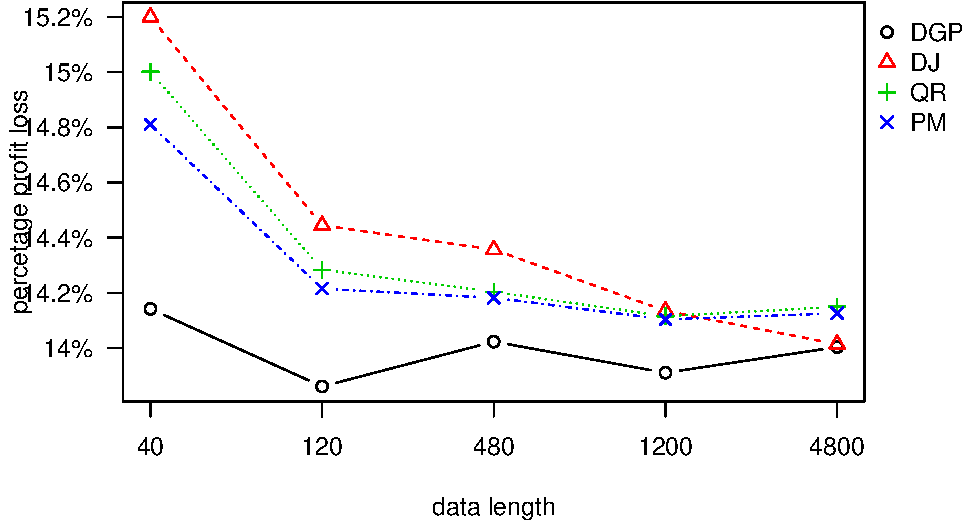
\includegraphics{linear-norm-plot_files/figure-latex/ppl0.63-1.pdf}

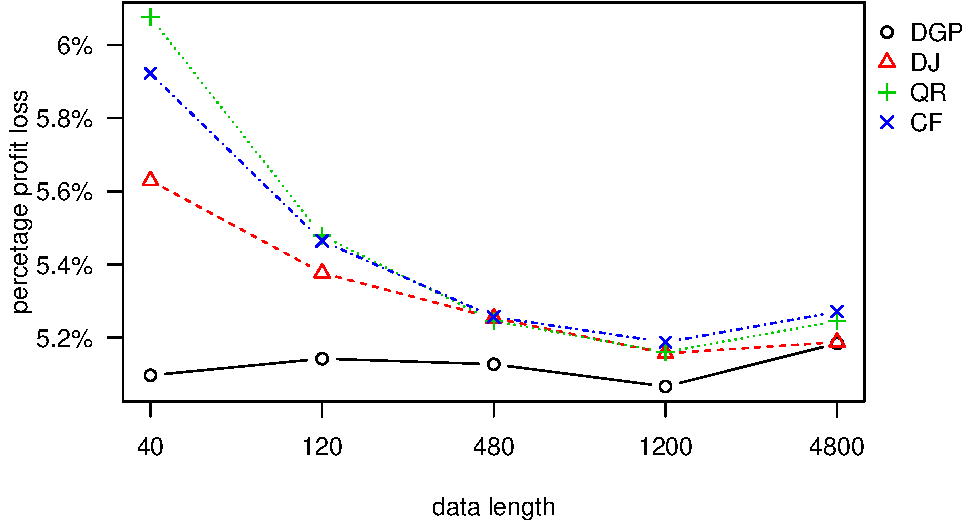
\includegraphics{linear-norm-plot_files/figure-latex/ppl0.3-1.pdf}

\begin{table}

\caption{\label{tab:inventory_error}Inventory Error}
\centering
\resizebox{\linewidth}{!}{
\begin{tabular}[t]{ccccccccccccc}
\toprule
\multicolumn{1}{c}{\textbf{ }} & \multicolumn{4}{c}{\textbf{Target service level=0.5}} & \multicolumn{4}{c}{\textbf{Target service level=0.63}} & \multicolumn{4}{c}{\textbf{Target service level=0.3}} \\
\cmidrule(l{3pt}r{3pt}){2-5} \cmidrule(l{3pt}r{3pt}){6-9} \cmidrule(l{3pt}r{3pt}){10-13}
Data size & DGP & disjoint & quantile & proposed & DGP & disjoint & quantile & proposed & DGP & disjoint & quantile & proposed\\
\midrule
\rowcolor{gray!6}  40 & -1.61 & 29.56 & -1.27 & -1.46 & -88.75 & -46.19 & -69.28 & -66.68 & 134.22 & 149.11 & 104.67 & 102.89\\
 & (200.74) & (221.15) & (218.1) & (215.86) & (200.02) & (222.48) & (216.76) & (214.36) & (198.14) & (220.03) & (216.95) & (214.71)\\
\rowcolor{gray!6}  120 & 2.29 & 14.11 & 2.11 & 2.22 & -75.26 & -62.02 & -69.67 & -68.33 & 114.94 & 126.39 & 106.52 & 104.91\\
 & (201.06) & (211.95) & (207.78) & (207.27) & (197.67) & (209.4) & (205.24) & (204.46) & (200.09) & (211.08) & (206.96) & (206.94)\\
\rowcolor{gray!6}  480 & -0.05 & 2.36 & 0.59 & 0.63 & -70.29 & -68.27 & -69.02 & -67.84 & 106.91 & 111.53 & 105.2 & 103.62\\
\addlinespace
 & (199.95) & (205.52) & (203.03) & (202.91) & (201.47) & (207.77) & (204.22) & (204.3) & (201.05) & (206.74) & (204.7) & (205.03)\\
\rowcolor{gray!6}  1200 & -2.1 & -0.47 & -2.03 & -2.02 & -68.94 & -67.98 & -68.87 & -67.75 & 106.83 & 110.18 & 106.81 & 105.2\\
 & (199.53) & (204.15) & (202.15) & (202.03) & (200.43) & (204.5) & (203.53) & (203.75) & (199.27) & (203.69) & (202.08) & (202.58)\\
\rowcolor{gray!6}  4800 & -1.88 & -1.51 & -1.87 & -1.9 & -66.43 & -65.99 & -66.96 & -65.77 & 107.34 & 107.88 & 108.2 & 106.74\\
 & (200.87) & (201.26) & (203.03) & (202.99) & (200.98) & (201.31) & (203.17) & (203.26) & (198.92) & (199.41) & (201.5) & (201.94)\\
\bottomrule
\end{tabular}}
\end{table}

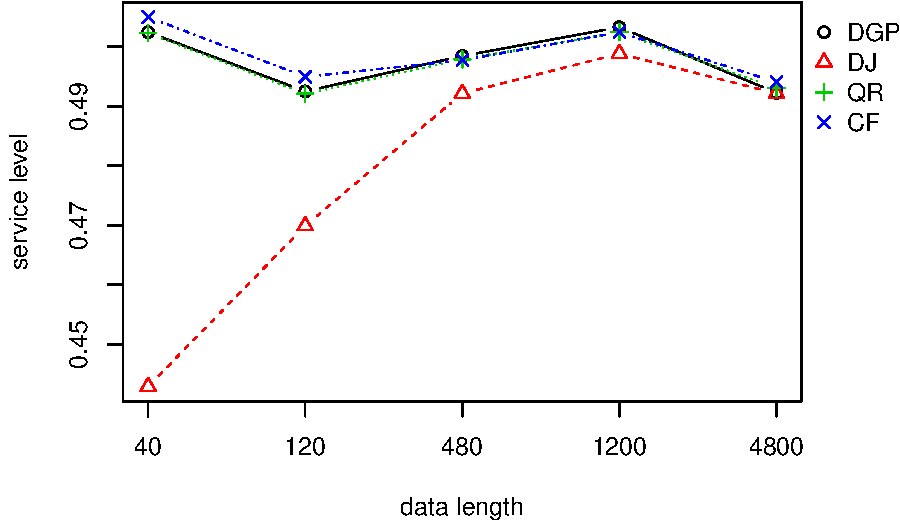
\includegraphics{linear-norm-plot_files/figure-latex/sl-1.pdf}
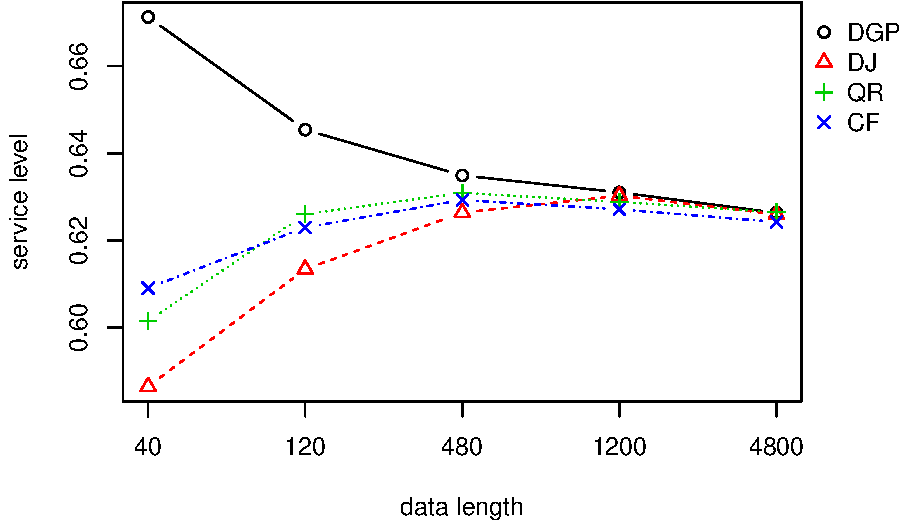
\includegraphics{linear-norm-plot_files/figure-latex/sl-2.pdf}
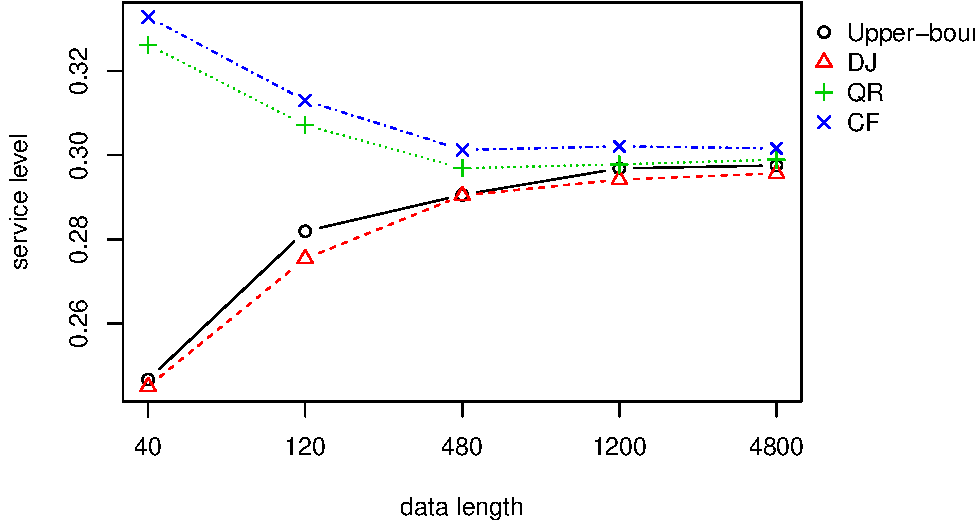
\includegraphics{linear-norm-plot_files/figure-latex/sl-3.pdf}
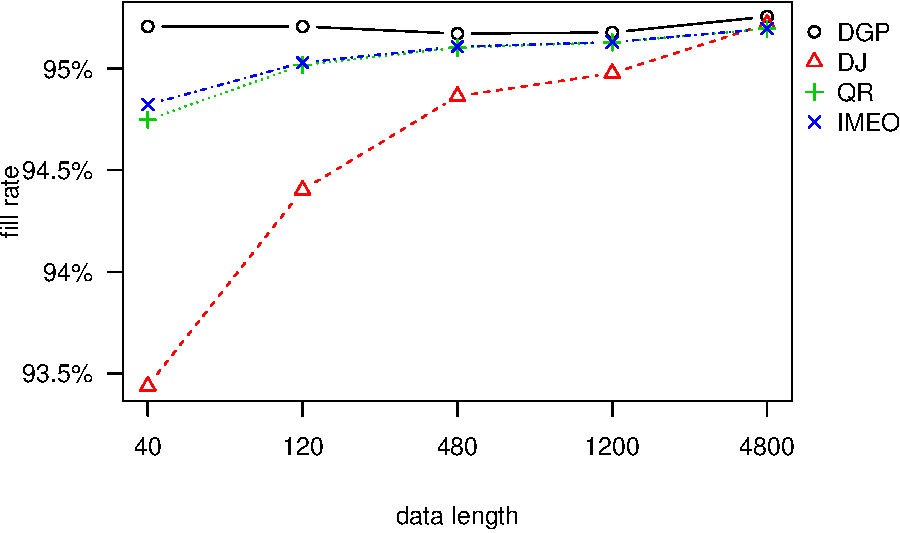
\includegraphics{linear-norm-plot_files/figure-latex/fr-1.pdf}
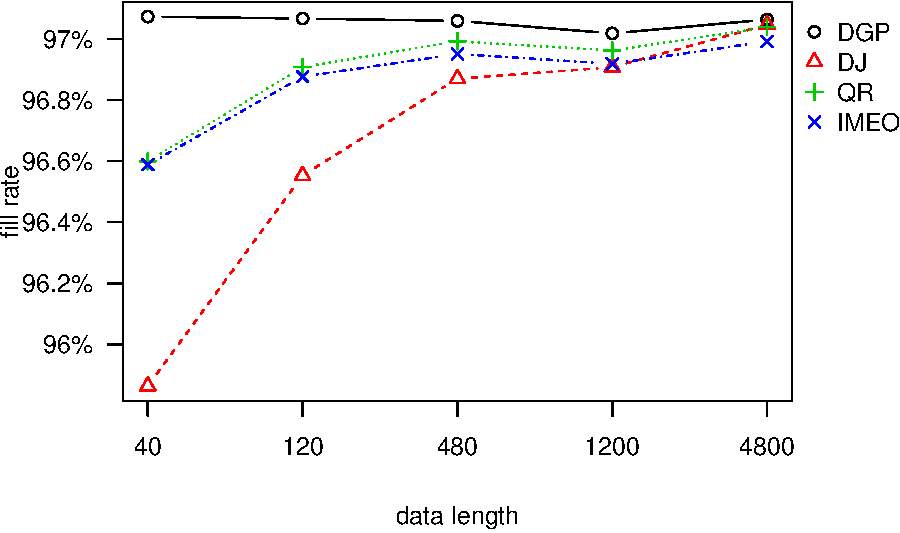
\includegraphics{linear-norm-plot_files/figure-latex/fr-2.pdf}
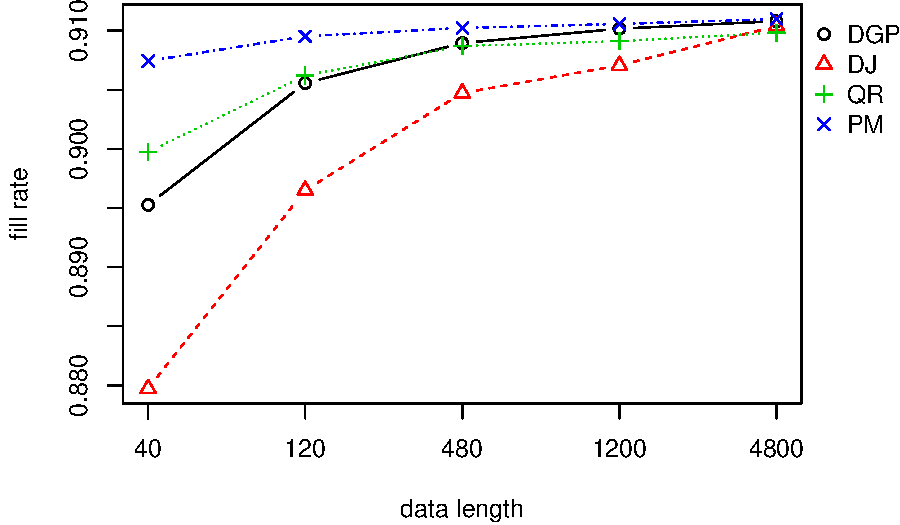
\includegraphics{linear-norm-plot_files/figure-latex/fr-3.pdf}

\begin{table}

\caption{\label{tab:Wilcoxon}p-value of Wilcoxon Test between data size 1200 and 4800}
\centering
\begin{tabular}[t]{ccccc}
\toprule
Target service level & DGP & disjoint & quantile & proposed\\
\midrule
\rowcolor{gray!6}  0.5 & 0.6383439 & 0.2627199 & 0.6170665 & 0.5686694\\
0.63 & 0.1649179 & 0.5483178 & 0.2374379 & 0.3680330\\
\rowcolor{gray!6}  0.3 & 0.8697539 & 0.4565893 & 0.9738829 & 0.9046732\\
\bottomrule
\end{tabular}
\end{table}

\textbackslash begin\{table\}

\textbackslash caption\{\label{tab:size0.3}Size effect (q=30\%)\}
\centering \resizebox{\linewidth}{!}{
\begin{tabular}[t]{ccccccccccccc}
\toprule
\multicolumn{1}{c}{\textbf{ }} & \multicolumn{4}{c}{\textbf{Percentage profit loss}} & \multicolumn{4}{c}{\textbf{Service level}} & \multicolumn{4}{c}{\textbf{Fill rate}} \\
\cmidrule(l{3pt}r{3pt}){2-5} \cmidrule(l{3pt}r{3pt}){6-9} \cmidrule(l{3pt}r{3pt}){10-13}
Data size & DGP & disjoint & quantile & proposed & DGP & disjoint & quantile & proposed & DGP & disjoint & quantile & proposed\\
\midrule
40 & 5.0\% & 5.6\% & 5.6\% & 5.5\% & 0.25 & 0.25 & 0.31 & 0.31 & 89.7\% & 88.2\% & 90.6\% & 90.8\%\\
120 & 5.1\% & 5.4\% & 5.3\% & 5.3\% & 0.28 & 0.27 & 0.30 & 0.31 & 90.6\% & 89.7\% & 90.8\% & 91.0\%\\
480 & 5.2\% & 5.3\% & 5.3\% & 5.3\% & 0.30 & 0.29 & 0.30 & 0.31 & 91.0\% & 90.5\% & 91.0\% & 91.1\%\\
1200 & 5.1\% & 5.2\% & 5.2\% & 5.2\% & 0.30 & 0.29 & 0.30 & 0.30 & 91.0\% & 90.7\% & 90.9\% & 91.1\%\\
4800 & 5.1\% & 5.1\% & 5.2\% & 5.2\% & 0.30 & 0.30 & 0.30 & 0.30 & 91.0\% & 90.9\% & 90.9\% & 91.0\%\\
\bottomrule
\end{tabular}} \textbackslash end\{table\}

\begin{table}[H]
\centering
\resizebox{\linewidth}{!}{
\begin{tabular}{ccccccccccccc}
\toprule
\multicolumn{1}{c}{\textbf{ }} & \multicolumn{4}{c}{\textbf{Percentage profit loss}} & \multicolumn{4}{c}{\textbf{Service level}} & \multicolumn{4}{c}{\textbf{Fill rate}} \\
\cmidrule(l{3pt}r{3pt}){2-5} \cmidrule(l{3pt}r{3pt}){6-9} \cmidrule(l{3pt}r{3pt}){10-13}
Target service level & DGP & disjoint & quantile & proposed & DGP & disjoint & quantile & proposed & DGP & disjoint & quantile & proposed\\
\midrule
\rowcolor{gray!6}  0.5 & 5.0\% & 5.4\% & 5.4\% & 5.3\% & 0.50 & 0.44 & 0.50 & 0.50 & 95.2\% & 93.5\% & 94.7\% & 94.8\%\\
0.63 & 14.1\% & 15.2\% & 15.0\% & 14.8\% & 0.67 & 0.58 & 0.63 & 0.62 & 97.5\% & 95.8\% & 96.6\% & 96.6\%\\
\rowcolor{gray!6}  0.3 & 5.0\% & 5.6\% & 5.6\% & 5.5\% & 0.25 & 0.25 & 0.31 & 0.31 & 89.7\% & 88.2\% & 90.6\% & 90.8\%\\
\bottomrule
\end{tabular}}
\end{table}

\begin{table}

\caption{\label{tab:level480}Target service level effect (n=480)}
\centering
\resizebox{\linewidth}{!}{
\begin{tabular}[t]{ccccccccc}
\toprule
\multicolumn{1}{c}{\textbf{ }} & \multicolumn{4}{c}{\textbf{Percentage profit loss}} & \multicolumn{4}{c}{\textbf{Service level}} \\
\cmidrule(l{3pt}r{3pt}){2-5} \cmidrule(l{3pt}r{3pt}){6-9}
Target service level & DGP & disjoint & quantile & proposed & DGP & disjoint & quantile & proposed\\
\midrule
\rowcolor{gray!6}  0.5 & 4.9\% & 5.0\% & 5.0\% & 5.0\% & 0.50 & 0.50 & 0.50 & 0.50\\
0.63 & 14.0\% & 14.4\% & 14.2\% & 14.2\% & 0.64 & 0.63 & 0.63 & 0.63\\
\rowcolor{gray!6}  0.3 & 5.2\% & 5.3\% & 5.3\% & 5.3\% & 0.30 & 0.29 & 0.30 & 0.31\\
\bottomrule
\end{tabular}}
\end{table}

\begin{table}[H]
\centering
\resizebox{\linewidth}{!}{
\begin{tabular}{ccccccccccccc}
\toprule
\multicolumn{1}{c}{\textbf{ }} & \multicolumn{4}{c}{\textbf{Percentage profit loss}} & \multicolumn{4}{c}{\textbf{Service level}} & \multicolumn{4}{c}{\textbf{Fill rate}} \\
\cmidrule(l{3pt}r{3pt}){2-5} \cmidrule(l{3pt}r{3pt}){6-9} \cmidrule(l{3pt}r{3pt}){10-13}
Target service level & DGP & disjoint & quantile & proposed & DGP & disjoint & quantile & proposed & DGP & disjoint & quantile & proposed\\
\midrule
\rowcolor{gray!6}  0.5 & 5.0\% & 5.0\% & 5.0\% & 5.0\% & 0.50 & 0.50 & 0.50 & 0.50 & 95.2\% & 95.2\% & 95.2\% & 95.2\%\\
0.63 & 14.0\% & 14.0\% & 14.1\% & 14.1\% & 0.63 & 0.63 & 0.63 & 0.63 & 97.0\% & 96.9\% & 96.9\% & 96.9\%\\
\rowcolor{gray!6}  0.3 & 5.1\% & 5.1\% & 5.2\% & 5.2\% & 0.30 & 0.30 & 0.30 & 0.30 & 91.0\% & 90.9\% & 90.9\% & 91.0\%\\
\bottomrule
\end{tabular}}
\end{table}

\end{document}
